
The pilot study reveals that hallucination detection method performance varies across benchmarks.

\subsubsection{Main Results}

\textbf{Table 1: Hallucination Detection AUROC (Pilot Study, N=20 samples per dataset)}

\begin{table}[htbp]
\centering
\resizebox{\columnwidth}{!}{%
\begin{tabular}{lll}
\toprule
Method & TruthfulQA & HaluEval \\
\midrule
Semantic Entropy & 0.289 [0.105, 0.526] & 0.551 [0.267, 0.800] \\
Self-Consistency & 0.474 [0.252, 0.687] & 0.444 [0.155, 0.733] \\
Gate Threshold & 0.55 & 0.55 \\
\bottomrule
\end{tabular}
}
\end{table}

Values in brackets are 95\% bootstrap confidence intervals.

\textbf{Observations:}

\begin{enumerate}
\item \textbf{One condition meets the gate threshold.} Semantic entropy achieves AUROC 0.551 on HaluEval, marginally exceeding the 0.55 threshold.
\end{enumerate}

\begin{enumerate}
\item \textbf{TruthfulQA shows inverted results for semantic entropy.} AUROC 0.289 is below random (0.5), indicating high-entropy responses were associated with truthful rather than hallucinated outputs in this pilot.
\end{enumerate}

\begin{enumerate}
\item \textbf{Self-consistency performs near random on both benchmarks.} AUROC values of 0.444 and 0.474 are statistically indistinguishable from chance given the wide confidence intervals.
\end{enumerate}

\begin{enumerate}
\item \textbf{Confidence intervals are wide and overlapping.} The small sample size (N=20) prevents statistically powered conclusions.
\end{enumerate}

\subsubsection{Gate Evaluation}

\textbf{Gate Result:} 1 of 4 conditions pass the AUROC > 0.55 threshold.

\begin{table}[htbp]
\centering
\resizebox{\columnwidth}{!}{%
\begin{tabular}{lll}
\toprule
Method & TruthfulQA & HaluEval \\
\midrule
Semantic Entropy & FAIL (0.289) & PASS (0.551) \\
Self-Consistency & FAIL (0.474) & FAIL (0.444) \\
\bottomrule
\end{tabular}
}
\end{table}

\subsubsection{Benchmark Sensitivity}

Method ranking differs across benchmarks in this pilot: semantic entropy outperforms self-consistency on HaluEval (0.551 vs 0.444), but the pattern reverses on TruthfulQA (0.289 vs 0.474). However, given the wide confidence intervals, this observation requires validation with larger samples.

\begin{figure}[htbp]
\centering
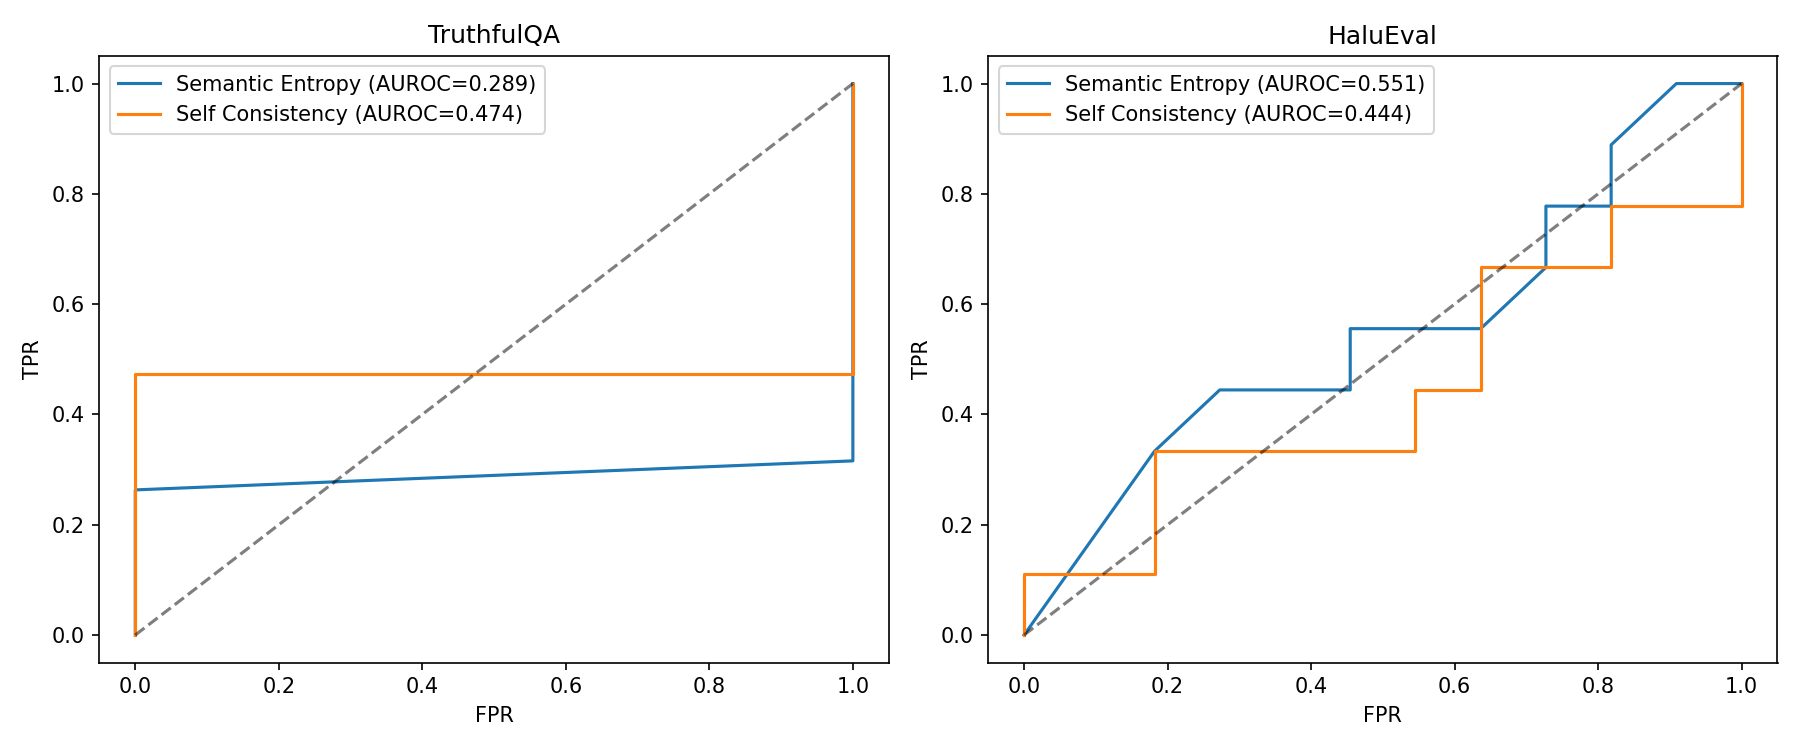
\includegraphics[width=\columnwidth]{figures/roc_curves.png}
\caption{ROC Curves}
\label{fig:roc_curves}
\end{figure}
\textit{Figure 1: ROC curves comparing detection methods across benchmarks.}

\begin{figure}[htbp]
\centering
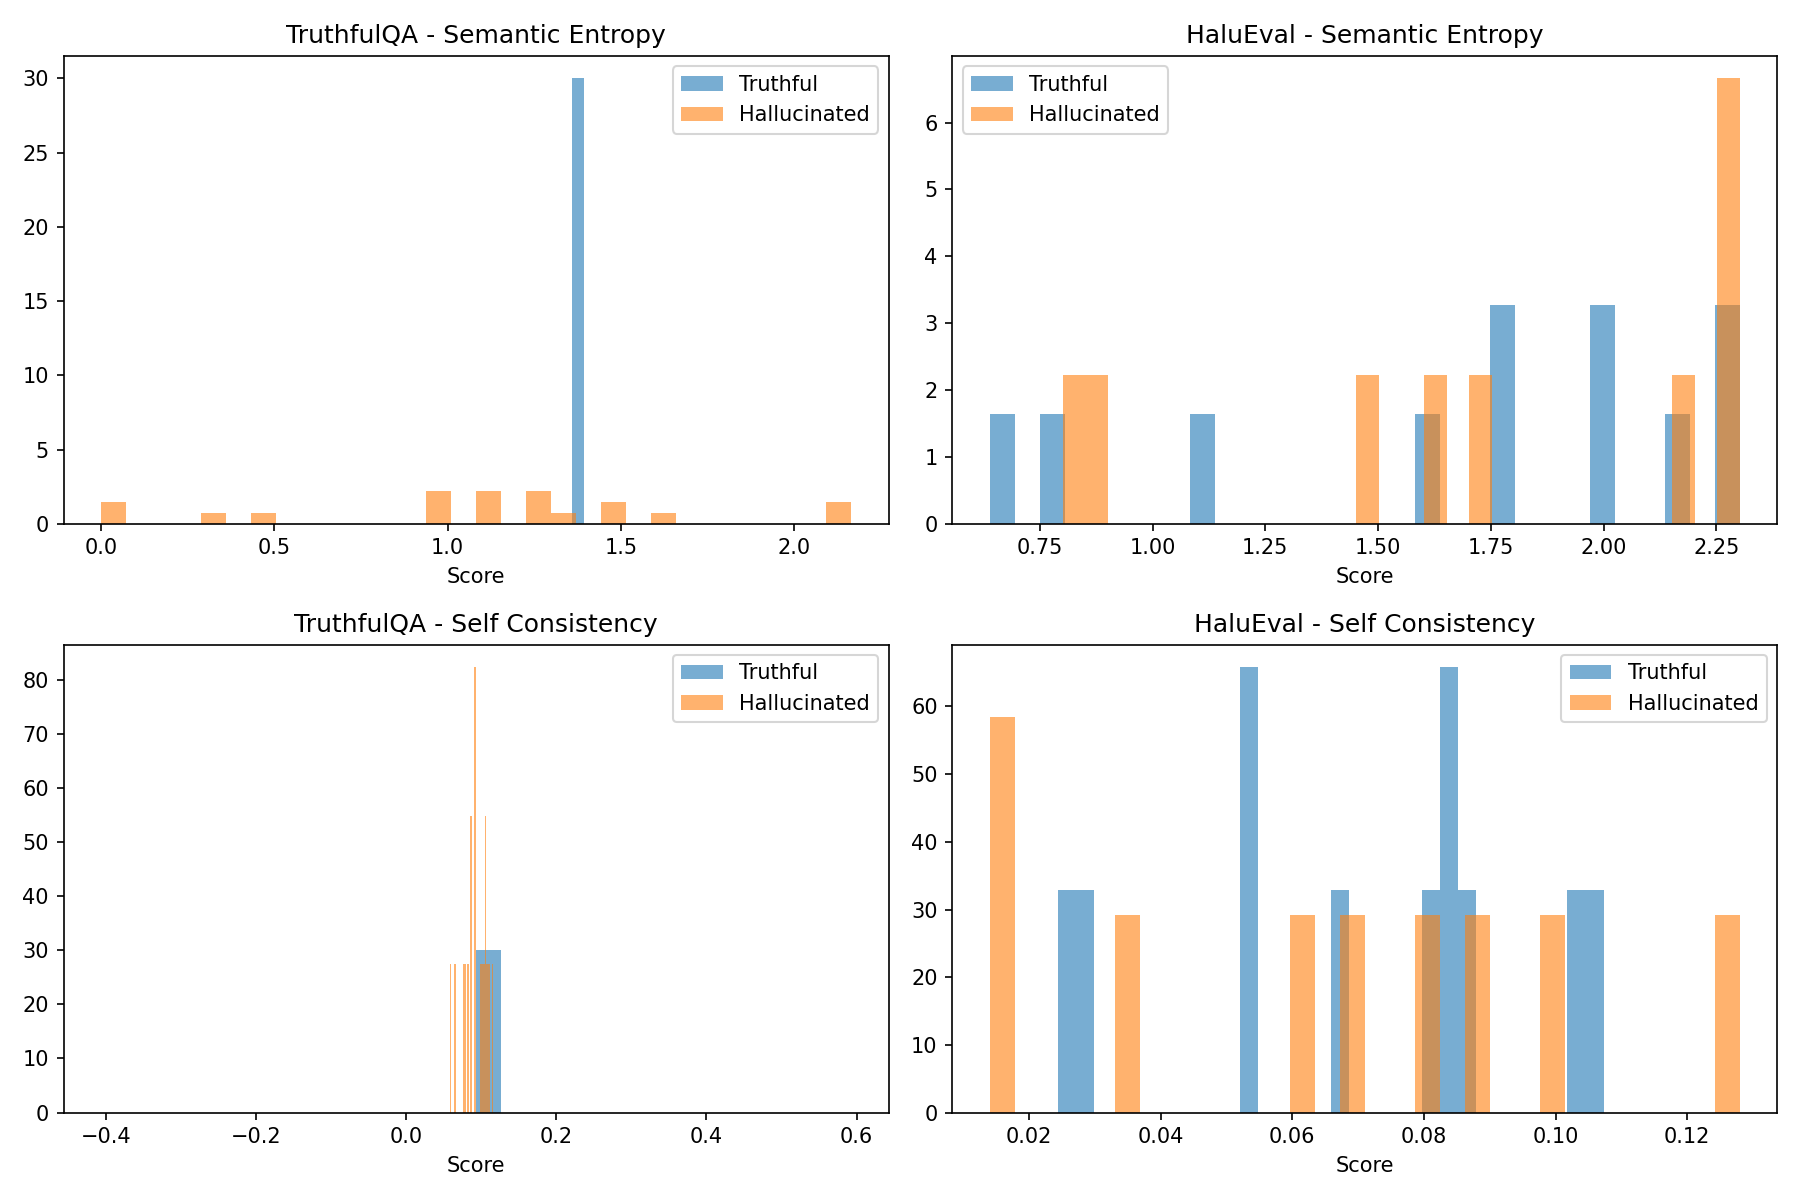
\includegraphics[width=\columnwidth]{figures/score_distributions.png}
\caption{Score Distributions}
\label{fig:score_distributions}
\end{figure}
\textit{Figure 2: Distribution of uncertainty scores for hallucinated vs truthful responses.}

\begin{figure}[htbp]
\centering
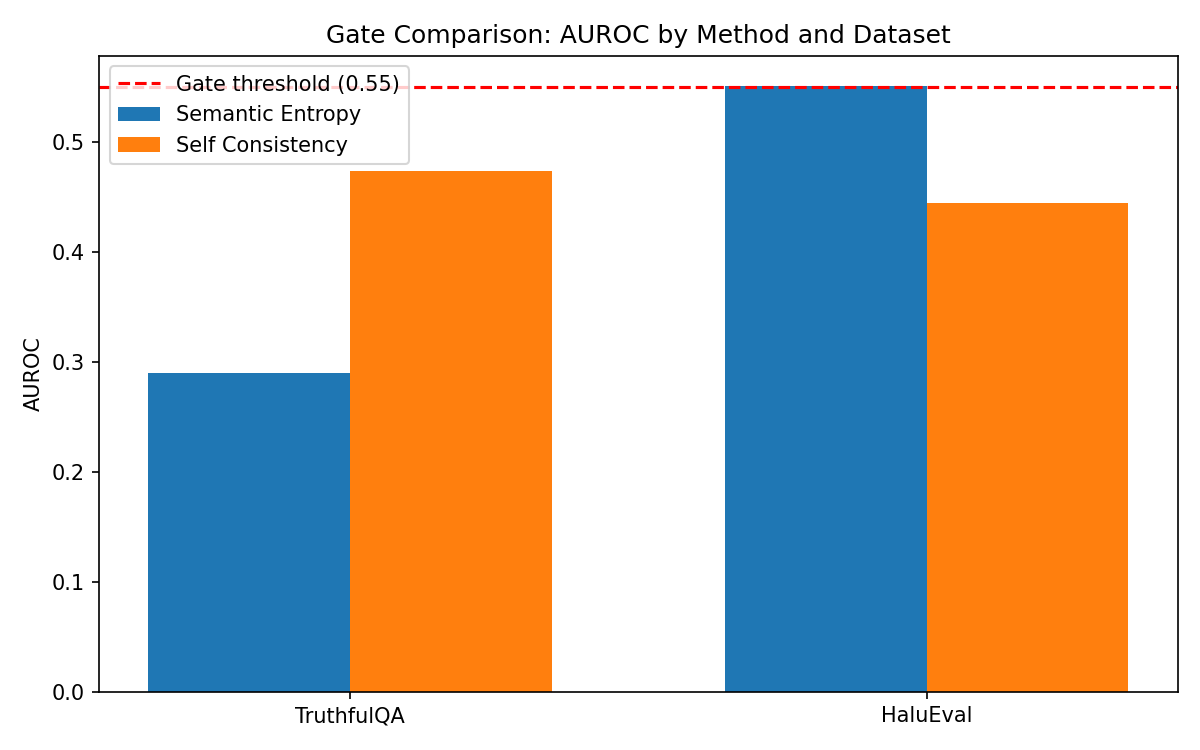
\includegraphics[width=\columnwidth]{figures/gate_comparison.png}
\caption{Gate Comparison}
\label{fig:gate_comparison}
\end{figure}
\textit{Figure 3: AUROC comparison against 0.55 gate threshold.}
